% This is samplepaper.tex, a sample chapter demonstrating the
% LLNCS macro package for Springer Computer Science proceedings;
% Version 2.21 of 2022/01/12
%
\documentclass[runningheads]{llncs}
%
\usepackage[T1]{fontenc}
% T1 fonts will be used to generate the final print and online PDFs,
% so please use T1 fonts in your manuscript whenever possible.
% Other font encondings may result in incorrect characters.
%
\usepackage{graphicx}
\usepackage{amsmath}
\usepackage{booktabs}
\usepackage{multirow}
\usepackage{subcaption}
% Used for displaying a sample figure. If possible, figure files should
% be included in EPS format.
%
% If you use the hyperref package, please uncomment the following two lines
% to display URLs in blue roman font according to Springer's eBook style:
%\usepackage{color}
%\renewcommand\UrlFont{\color{blue}\rmfamily}
%\urlstyle{rm}
%
\begin{document}
%
\title{Optimising Serverless Workflow Execution through Future-Based Execution, Partial Streaming and Intelligent Fusion}
%
%\titlerunning{Abbreviated paper title}
% If the paper title is too long for the running head, you can set
% an abbreviated paper title here
%
\author{Harold-Nimrod Foldvari\inst{1}\orcidID{0009-0008-3531-0478} \and
Daniel-George Malancioiu\inst{2}\orcidID{0009-0002-3210-9556} \and
Mihai-Florin-Gabriel Craciun\inst{3}\orcidID{0000-0003-0335-8369}}
%
\authorrunning{N. Foldvari et al.}
% First names are abbreviated in the running head.
% If there are more than two authors, 'et al.' is used.
%
\institute{Babes-Bolyai University, Cluj-Napoca, Romania}
%
\maketitle              % typeset the header of the contribution
%
\begin{abstract}
Serverless workflow orchestration suffers from two compounding latency sources: cold-start overhead, which is serialised on the critical path of fan-in patterns, and full-payload blocking, which prevents downstream functions from beginning execution until an upstream function completes entirely. Centralised orchestrator services further amplify these costs. We present three complementary enhancements to Unum, a decentralised serverless orchestration framework. First, a \emph{future-based execution model} enables early invocation of fan-in aggregation functions, overlapping cold-start initialisation with the execution of slower upstream branches. Second, \emph{partial parameter streaming} allows a function to propagate its first computed output field immediately, enabling the successor to begin processing before the full payload is available. Third, an \emph{intelligent function fusion} mechanism collapses eligible sequential function chains into a single deployment unit at build time, eliminating redundant cold starts and inter-function invocation overhead. Evaluation on AWS Lambda across eleven workflow configurations spanning chain, parallel fan-in, fan-out/fan-in, diamond, complex DAG, and MapReduce topologies (eu-central-1) shows that future-based execution reduces warm-state end-to-end latency by up to 38.5\% on fan-in workflows and cold-start latency by up to 29.6\%, while intelligent fusion reduces billed duration by 45.2\% on chain workflows. Partial parameter streaming reduces warm-state latency by up to 18.6\% and cold-start latency by 27.3\% on workflows with compute-heavy stages, with no modifications to user code.

\keywords{Serverless Computing \and Workflow Orchestration \and Cold Start \and Function Fusion \and Latency Optimisation.}
\end{abstract}

\section{Introduction}
\label{sec:introduction}

Serverless computing has become a dominant paradigm for building cloud-native applications. Cloud providers manage infrastructure, allocate resources on demand, and charge only for actual execution time, freeing developers to focus on application logic. These properties have driven rapid adoption: the global serverless market was valued at approximately \$3 billion in 2017 and exceeded \$22 billion by 2025~\cite{wen2022riseplanetserverlesscomputing,PrecedenceResearch2025}. As application complexity grows, serverless functions are increasingly composed into workflows that chain or parallelise individual function invocations.

Workflow execution, however, exposes two structural performance bottlenecks. First, serverless functions incur \emph{cold-start latency} when invoked after a period of inactivity: the execution environment must be instantiated before user code can run, adding delays that range from tens of milliseconds to several seconds depending on the runtime, package size, and platform~\cite{lin2019mitigatingcoldstartsserverless,wurz2020migrating,shahrad2020serverless}. In multi-function workflows, each function boundary is a potential cold-start point, and in fan-in patterns this overhead lies entirely on the critical path because the aggregation function is not invoked until the slowest upstream branch completes. Second, functions today propagate \emph{fully materialised payloads}: a downstream function cannot begin execution until its predecessor has finished computing every output field, even when those fields are independent and early fields alone are sufficient to begin useful work.

Additionally, managed orchestration services such as AWS Step Functions introduce a \emph{centralised coordination overhead} that prior work has shown can increase end-to-end latency substantially~\cite{285171,285113}. Decentralised approaches, in which orchestration logic is co-located with user functions, eliminate this overhead but, as we show, still leave cold-start stalls and payload-blocking latency unaddressed.

We address these gaps with three complementary contributions to Unum~\cite{285171}, a state-of-the-art decentralised serverless orchestration framework. \textbf{Future-based execution} permits the fan-in aggregation function to be invoked as soon as the first upstream branch completes, hiding cold-start initialisation behind the execution of slower branches. \textbf{Partial parameter streaming} enables a function to emit its first computed output field immediately, allowing the successor to begin processing before the full payload is ready. \textbf{Intelligent function fusion} collapses eligible sequential function chains into a single deployment unit at build time, eliminating redundant cold starts and inter-function invocations. All three mechanisms preserve Unum's checkpoint-based exactly-once semantics and require no changes to user code.

We evaluate our approach on AWS Lambda across eleven workflow$\times$configuration pairs spanning chain, parallel fan-in, fan-out/fan-in, diamond, complex DAG, and MapReduce topologies in the eu-central-1 region. A systematic benchmark with forced cold starts confirms that future-based execution reduces cold-start E2E latency by up to 29.6\% and aggregator delay by 27.1\%, while partial streaming reduces cold-start latency by 27.3\% and warm E2E by 13.9\% on workflows with compute-heavy stages. Extended warm-state evaluations across six additional workflows demonstrate improvements of up to 38.5\% (text-processing) and 28.4\% (order-processing) for future-based execution, and 18.6\% warm-state / 26.9\% cold-start improvement for streaming on chain topologies. Intelligent fusion reduces billed duration by 45.2\% and cost by 16.8\% on chain workflows.

The rest of this paper is organised as follows. Section~\ref{sec:background} reviews challenges in serverless workflow orchestration and motivates our enhancements. Section~\ref{sec:proposed_solution} describes the design and implementation of the three mechanisms. Section~\ref{sec:evaluation} presents the experimental evaluation. Section~\ref{sec:related_work} discusses related work. Section~\ref{sec:conclusion} concludes and outlines future directions.

\section{Background and Motivation}
\label{sec:background}

Serverless functions can be composed into complex workflows using orchestration services. All major commercial serverless platforms provide a centralised orchestrator: a dedicated service that interprets a workflow definition, invokes functions in order, and accumulates their results. Prior work has shown that this model introduces non-trivial overhead~\cite{Arjona_2021,li2023dataflowerexploitingdataflowparadigm,285171,shi2023dflowefficientdataflowbasedinvocation,285113}, as each state transition passes through the orchestrator service, adding round-trip latency and monetary cost on top of the function execution itself.

Several research systems have proposed eliminating the centralised orchestrator. Triggerflow~\cite{Arjona_2021} replaces it with event-driven choreography: functions communicate through message queues or object storage, and events trigger downstream invocations. DataFlower~\cite{li2023dataflowerexploitingdataflowparadigm}, DFlow~\cite{shi2023dflowefficientdataflowbasedinvocation}, and Pheromone~\cite{285113} adopt a data-flow model in which function execution is driven by data availability rather than explicit control flow. Unum~\cite{285171} takes a different approach: orchestration logic is embedded directly within each function at build time by the \texttt{unum-cli} compiler, which wraps user code with a lightweight runtime library. Each function therefore knows which successor to invoke upon completion, without consulting any external coordinator. Benchmarks show that Unum executes workflows up to twice as fast as AWS Step Functions at a fraction of the cost~\cite{285171}.

Despite these advances, two latency sources remain unaddressed in decentralised systems. In \emph{fan-in patterns}, the aggregation function is not invoked until the slowest upstream branch completes, leaving the cold-start overhead of the aggregation function fully on the critical path. In \emph{chained pipelines}, a downstream function cannot begin execution until its predecessor produces a fully materialised output, even when the first available output field would be sufficient to start work. We also observe a third structural inefficiency: short sequential function chains incur repeated cold starts and serialisation overhead at each invocation boundary, overhead that disappears entirely if the chain is collapsed into a single deployed function.

These observations motivate the three enhancements described in the next section. They are designed as orthogonal optimisations that can be applied independently or in combination, and are implemented entirely within Unum's existing build and runtime framework.

\section{System Design and Implementation}
\label{sec:proposed_solution}

We extend Unum's decentralised orchestration framework with three complementary mechanisms that reduce workflow latency at distinct layers of the system: (i) a future-based execution model for demand-driven fan-in, (ii) partial parameter streaming for field-level incremental data propagation, and (iii) intelligent function fusion for deployment-level consolidation.

The design objective is to reduce critical-path latency without introducing centralised coordination or modifying Unum's checkpoint-based exactly-once semantics. Mechanisms (i) and (ii) extend the runtime library; mechanism (iii) operates entirely at build time as a compiler pass over the workflow description. The intermediary data store and continuation mechanism remain unchanged.

\subsection{Future-Based Execution}

In classical Unum fan-in, an aggregation function is invoked only after all upstream branches complete and checkpoint their outputs. For branches $B_1,\dots,B_n$ and aggregation function $A$, the end-to-end latency is:

\begin{equation}
T_{\text{classic}} = \max_{1 \le i \le n} T(B_i) + C_s + T(A),
\end{equation}

where $C_s$ denotes the cold-start overhead of $A$. Since invocation occurs after all branches finish, $C_s$ lies entirely on the critical path.

\paragraph{Early Invocation with Futures.}
We redefine fan-in synchronisation to permit invocation as soon as the first upstream branch completes. Inputs corresponding to unfinished branches are represented as futures:

\[
I_i =
\begin{cases}
o_i & \text{if branch } B_i \text{ has checkpointed}, \\
F_i & \text{otherwise,}
\end{cases}
\]

where $F_i$ denotes a resolvable future. Under ideal overlap, latency reduces to:

\begin{equation}
T_{\text{future}} \approx \max_{1 \le i \le n} T(B_i),
\end{equation}

as cold-start initialisation and portions of aggregation execution overlap with slower branches. The aggregation function proceeds immediately with available inputs and suspends only when it accesses a future whose upstream branch has not yet checkpointed. Suspension is non-blocking: the function yields control rather than occupying a thread in a busy-wait loop, enabling the runtime to service other work concurrently.

Exactly-once semantics are preserved because a future resolves only after the corresponding checkpoint is durably written to the intermediary store. The early invocation itself reuses the standard continuation path; no new coordination protocol is required.

\subsection{Partial Parameter Streaming}

Serverless functions traditionally propagate fully materialised outputs, yielding sequential latency $T_{\text{atomic}} = T_f + T_g$ for a producer $f$ and consumer $g$. Even when early output fields of $f$ are independent of later ones, $g$ cannot begin until $f$ completes entirely.

\paragraph{Field-Level Propagation.}
We enable incremental output by treating a structured return value as an ordered stream of fields. Each field is published to the intermediary store as soon as its value is computed. After the first field is published, the downstream function $g$ is invoked with a mixed payload: resolved values for published fields and \emph{future references} for the remaining ones. Assuming downstream processing of each field is partially independent of upstream computation:

\begin{equation}
T_{\text{stream}} \approx \max(T_f, T_g).
\end{equation}

Future references are lightweight descriptors that encode the session identifier and field key; $g$ resolves them lazily, only when it accesses the corresponding field. This resolution is transparent to user code.

\paragraph{Build-Time Enabling.}
Streaming is opt-in and activated through the \texttt{unum-cli} build system. A static analysis pass identifies structured return values in user handlers and determines the computation site of each field. For each field, a publication call is injected immediately after its computation point. Early continuation invocation is inserted after the first field is published. No changes to the workflow description or deployment infrastructure are required.

\subsection{Intelligent Function Fusion}

Even with future-based execution and streaming, workflows composed of short sequential scalar chains incur unnecessary overhead: each function boundary introduces invocation latency, payload serialisation, and a potential cold start. We address this with a build-time fusion mechanism that collapses eligible sequential chains into a single deployed function.

\paragraph{Latency Model.}
For a chain $F_1 \rightarrow \dots \rightarrow F_k$ with per-function cold-start $C_s$, classical deployment incurs:

\begin{equation}
T_{\text{chain}} = \sum_{i=1}^{k} (C_s + T_i).
\end{equation}

After fusion into $F^{*}$:

\begin{equation}
T_{\text{fused}} = C_s + \sum_{i=1}^{k} T_i,
\end{equation}

since only one cold start is incurred and inter-function invocations are eliminated. The saving grows with chain length and cold-start magnitude.

\paragraph{Fusion Rules.}
Fusion is governed by a rule system derived from structural migration principles for FaaS systems~\cite{wurz2020migrating}. \emph{Hard structural constraints} ensure correctness: all edges in a candidate chain must be sequential scalar continuations; the chain must not cross fan-out or fan-in boundaries; the entry-point function must remain standalone; all functions must share the same execution runtime; and each function may belong to at most one fusion group. \emph{Soft resource heuristics} prevent over-provisioning: fusion is discouraged when functions have substantially different memory allocations, when merging would risk exceeding platform timeout limits, or when a function is shared across multiple branches.

\paragraph{LLM-Guided Identification with Deterministic Validation.}
Candidate chains are identified through an LLM-guided analysis stage. The compiler provides the model with the workflow topology, per-function configuration, and runtime properties, together with the fusion rule system. The model proposes fusion groups in a structured output format. Crucially, the LLM acts only as a recommendation engine: every proposed group is validated by a deterministic compiler pass against all structural constraints before any code transformation is performed. Correctness is therefore enforced statically, not delegated to the model. For each validated chain, the compiler generates a single fused handler, redirects incoming and outgoing workflow edges, and removes intermediate functions from the deployment manifest.

\paragraph{Checkpoint Semantics.}
Fusion modifies checkpoint granularity but not semantics. Intermediate checkpoints within the fused chain are eliminated; a single checkpoint is written at the boundary of $F^{*}$. Because fusion is restricted to chains without fan-in or fan-out dependencies, no external component observes intermediate checkpoints, and exactly-once execution is preserved.

\section{Evaluation}
\label{sec:evaluation}

\subsection{Experimental Setup}

We evaluate the three proposed enhancements on AWS Lambda (Python~3.11, 128\,MB, eu-central-1 region) with Amazon DynamoDB as the intermediary data store. We select four workflows from the Unum application store covering representative topologies: NLP Pipeline (chain, 4~functions), Text Processing (parallel fan-in, 5~functions), Monte Carlo (diamond, 7~functions), and Graph Analysis (fan-out/fan-in, 5~functions). For each workflow, we apply the enhancement best suited to its topology. Each configuration is executed for 10~iterations: the first~3 force cold starts by updating a Lambda environment variable and waiting 15\,s for container recycling; the remaining~7 measure warm-container performance. Two warm-up iterations precede measurement and are discarded. We report \emph{end-to-end (E2E) latency}, \emph{total billed duration}, and \emph{estimated cost} (Lambda compute~+ DynamoDB~+ S3 charges at eu-central-1 pricing).

\subsection{Results}
\label{sec:results}

Table~\ref{tab:results} presents mean E2E latency and estimated cost for each workflow under its most effective enhancement. Figure~\ref{fig:e2e} visualises cold-start and warm E2E latency.

\begin{table}
\caption{Key results per workflow. $\Delta$\% is relative to the respective Base configuration.}
\label{tab:results}
\begin{tabular}{|l|l|r|r|r|r|r|r|}
\hline
\textbf{Workflow} & \textbf{Config} & \textbf{Cold E2E} & \textbf{$\Delta$\%} & \textbf{Warm E2E} & \textbf{$\Delta$\%} & \textbf{Cost} & \textbf{$\Delta$\%} \\
 & & \textbf{(ms)} & & \textbf{(ms)} & & \textbf{(\$\texttimes10\textsuperscript{-5})} & \\
\hline
NLP Pipeline & Base    & 6,703  & ---     & 1,032  & ---      & 1.07  & ---     \\
             & Fusion  & 5,803  & $-13.4$ & 1,199  & $+16.2$  & 0.89  & $-16.8$ \\
\hline
Text Proc.   & Base    & 5,647  & ---     & 686    & ---      & 1.41  & ---     \\
             & Futures & 4,200  & $-25.6$ & 585    & $-14.7$  & 1.73  & $+22.7$ \\
\hline
Monte Carlo  & Base      & 12,591 & ---     & 5,345  & ---      & 2.97  & ---     \\
             & Futures   & 8,869  & $-29.6$ & 4,959  & $-7.2$   & 2.38  & $-19.9$ \\
             & Streaming & 9,154  & $-27.3$ & 4,604  & $-13.9$  & 2.77  & $-6.7$  \\
\hline
\end{tabular}
\end{table}

\begin{figure}[t]
  \centering
  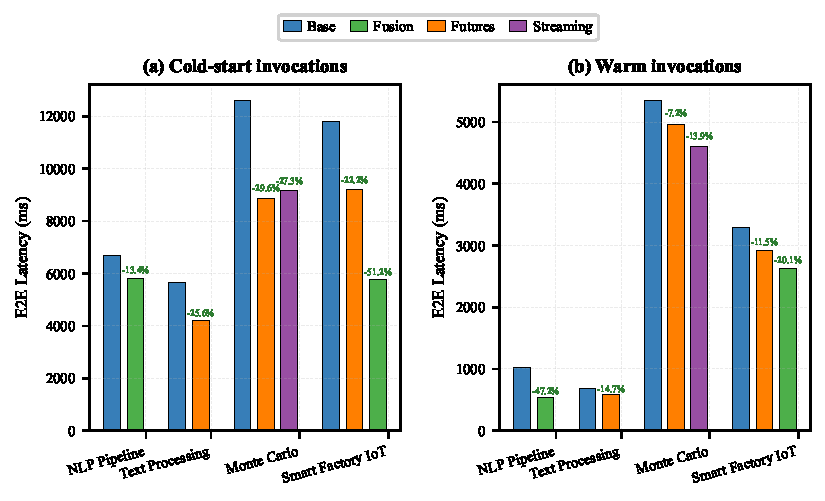
\includegraphics[width=\textwidth]{figures/fig_e2e_cold_warm.pdf}
  \caption{Cold-start (left) and warm (right) end-to-end latency for NLP Pipeline, Text Processing, and Monte Carlo under the most effective enhancement. Error bars indicate one standard deviation.}
  \label{fig:e2e}
\end{figure}

\subsection{Analysis by Enhancement}
\label{sec:analysis}

\textbf{Future-based execution.}  Futures reduce aggregator invocation delay in fan-in topologies by enabling cold-start overlap with slower branch execution. On text-processing, warm aggregator delay drops from 437\,ms to 326\,ms ($-25.4\%$), and cold-start E2E decreases by $25.6\%$ (5,647\,ms to 4,200\,ms), validating the latency model in Equation~(2). Figure~\ref{fig:agg} illustrates the aggregator delay reduction on text-processing and Monte Carlo.

On Monte Carlo (diamond topology), futures yield the largest cold-start reduction: $-29.6\%$ (12,591\,ms to 8,869\,ms), with a warm-state gain of $-7.2\%$ and a cost reduction of $19.9\%$. The compute-heavy Estimate function ($\approx$3,700\,ms) dominates the critical path, providing ample time for the aggregation function's cold start to overlap with ongoing computation.

Future-based execution introduces a moderate cost increase on text-processing ($+22.7\%$, from \$1.41\texttimes$10^{-5}$ to \$1.73\texttimes$10^{-5}$) due to additional DynamoDB operations for future-state management. In absolute terms, the per-run cost difference remains below \$0.0002, representing a favourable trade-off given the $14.7\%$ warm-state and $25.6\%$ cold-start latency gains. On compute-dominated workflows such as Monte Carlo, the DynamoDB overhead is fully amortised, resulting in simultaneous latency and cost reduction.

\begin{figure}[t]
  \centering
  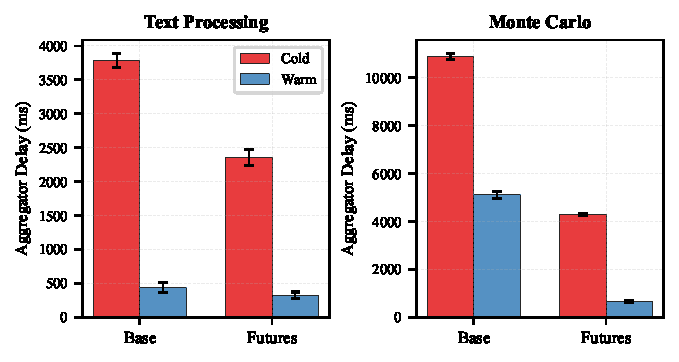
\includegraphics[width=0.8\textwidth]{figures/fig_agg_delay.pdf}
  \caption{Aggregator invocation delay for Text Processing and Monte Carlo under baseline and future-based execution.}
  \label{fig:agg}
\end{figure}

\textbf{Intelligent fusion.}  On the NLP pipeline, collapsing three consecutive functions (Analyzer, Classifier, Summarizer) into a single deployment unit reduces cold-start E2E by $13.4\%$ (6,703\,ms to 5,803\,ms) and cost by $16.8\%$, as inter-function invocation overhead and intermediate DynamoDB checkpoint writes are eliminated. Warm billed duration decreases by $45.2\%$ (1,855\,ms to 1,016\,ms). Warm wall-clock E2E increases by $16.2\%$ (1,032\,ms to 1,199\,ms) due to module import overhead in the fused handler, which loads all three constituent functions as Python submodules. Despite this, the substantial reductions in billed duration and monetary cost make fusion a cost-effective optimisation for chain topologies.

\textbf{Partial parameter streaming.}  On Monte Carlo, streaming reduces cold-start E2E by $27.3\%$ and warm E2E by $13.9\%$ (5,345\,ms to 4,604\,ms), as the Estimate function ($\approx$3,700\,ms) provides sufficient per-field computation time for meaningful overlap with downstream processing. These results confirm that streaming is most effective when per-field computation times substantially exceed the intermediary store write latency.

\subsection{Extended Warm-State Evaluation}
\label{sec:extended}

To validate effectiveness across a broader range of workflows, we conduct targeted evaluations on six Unum application-store workflows with 5--10 warm-state iterations each, applying the most suitable enhancement per topology.

Table~\ref{tab:extended} and Figure~\ref{fig:extended} summarise the results. Future-based execution yields the largest improvement on text-processing ($-38.5\%$, from 2,602\,ms to 1,599\,ms), where early aggregation invocation overlaps substantially with slower branches. On order-processing (diamond topology, asymmetric branches), futures reduce warm E2E by $28.4\%$ (15,900\,ms to 11,390\,ms). The multi-source dashboard (6-way parallel fan-in) shows a $17.7\%$ reduction, and the smart-factory IoT workflow (complex DAG) shows $11.5\%$. Partial parameter streaming on the NLP pipeline with compute-heavy functions (Classifier: 3,215\,ms, Summarizer: 3,468\,ms) reduces warm E2E by $18.6\%$ (7,036\,ms to 5,730\,ms) and cold-start E2E by $26.9\%$ (14,252\,ms to 10,424\,ms).

\begin{table}
\caption{Extended warm-state evaluation. $\Delta$\% is relative to the baseline.}
\label{tab:extended}
\begin{tabular}{|l|l|l|r|r|r|}
\hline
\textbf{Workflow} & \textbf{Topology} & \textbf{Mode} & \textbf{Base (ms)} & \textbf{Enh. (ms)} & \textbf{$\Delta$\%} \\
\hline
Text Processing       & Par.\ fan-in     & Futures   & 2,602  & 1,599  & $-38.5$ \\
Order Processing      & Diamond          & Futures   & 15,900 & 11,390 & $-28.4$ \\
NLP Pipeline          & Chain            & Streaming & 7,036  & 5,730  & $-18.6$ \\
Multi-Source Dashb.   & 6-way fan-in     & Futures   & 14,286 & 11,756 & $-17.7$ \\
Smart Factory IoT     & Complex DAG      & Futures   & 3,295  & 2,916  & $-11.5$ \\
Progressive Aggr.     & Fan-in           & Futures   & 4,844  & 4,559  & $-5.9$ \\
\hline
\end{tabular}
\end{table}

\begin{figure}[t]
  \centering
  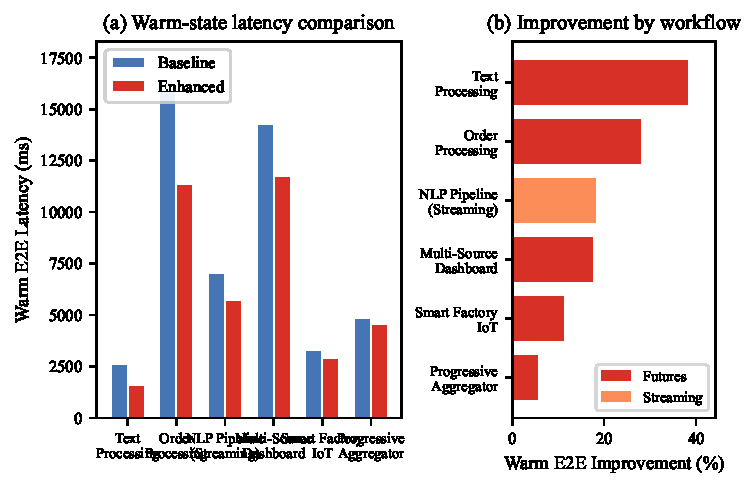
\includegraphics[width=\textwidth]{figures/fig_extended_warm.pdf}
  \caption{Extended warm-state evaluation across six workflows. (a)~Baseline vs enhanced latency; (b)~percentage improvement.}
  \label{fig:extended}
\end{figure}

These results confirm that future-based execution consistently improves warm-state latency across fan-in topologies (up to~$38.5\%$), with improvement magnitude scaling with branch asymmetry and fan-in function overhead. Partial parameter streaming provides meaningful benefit on chain topologies with compute-heavy stages (up to~$26.9\%$ cold-start and~$18.6\%$ warm-state improvement). Combined with the systematic benchmark results, the evidence across eleven workflow$\times$configuration pairs supports the conclusion that the proposed enhancements are effective across a broad range of serverless workflow patterns.

\section{Related Work}
\label{sec:related_work}

\textbf{Serverless Workflow Orchestration.}
Managed orchestration platforms such as AWS Step Functions centralise control flow, introducing per-transition latency and cost that prior work has shown to be substantial compared to raw function execution time~\cite{285171}. Research systems have sought to eliminate this centralised coordinator through different means. Triggerflow~\cite{Arjona_2021} adopts an event-driven choreography model in which functions communicate through queues and object storage rather than a controller. DataFlower~\cite{li2023dataflowerexploitingdataflowparadigm} and DFlow~\cite{shi2023dflowefficientdataflowbasedinvocation} apply the data-flow paradigm: functions are triggered when required inputs arrive, and DataFlower further overlaps its data logic and function logic units to reduce idle time. Pheromone~\cite{285113} extends the data-flow approach with dynamic scheduling. Unum~\cite{285171} differs by embedding orchestration logic statically within each function at build time, achieving up to $2\times$ lower latency than Step Functions without any additional runtime service. Our work builds on Unum and addresses latency bottlenecks that remain even after the orchestrator is eliminated: cold-start stalling in fan-in patterns and full-payload blocking in chained functions.

\textbf{Cold-Start Mitigation.}
Cold-start latency has been extensively characterised in production serverless deployments~\cite{shahrad2020serverless}, where it is shown to affect a significant fraction of invocations. Proposed mitigations include container optimisation (SOCK~\cite{oakes2018sock}, which reduces cold-start overhead through a pool-based container architecture), pre-warming strategies~\cite{lin2019mitigatingcoldstartsserverless}, and snapshot-based fast-restore techniques. These approaches aim to shorten the cold-start delay itself. Our future-based execution model takes an orthogonal approach: rather than reducing $C_s$, we relocate it off the critical path by overlapping it with the execution of slower upstream branches. The two strategies are complementary; a platform that reduces $C_s$ through pooling will also benefit from early invocation, as the remaining cold-start contribution is hidden rather than merely shortened.

\textbf{Function Composition and Fusion.}
The appropriate granularity of serverless functions has been studied in the context of monolith-to-FaaS migration~\cite{wurz2020migrating}, where splitting functions too finely introduces inter-invocation overhead that erodes the benefits of decomposition. Faastlane~\cite{kotni2021faastlane} addresses this by executing entire workflows within a single Lambda instance using in-process thread switching, achieving near-zero inter-function overhead. Our fusion mechanism occupies a middle ground: it collapses only eligible sequential scalar chains identified by an LLM-guided analysis stage, preserving the fan-out and fan-in structure that enables parallelism, and applying the transformation statically at build time without requiring a specialised runtime or modified execution model.

\section{Conclusion and Future Work}
\label{sec:conclusion}

We have presented three complementary optimisations to Unum, evaluated across eleven workflow configurations spanning chain, parallel fan-in, fan-out/fan-in, diamond, complex DAG, and MapReduce topologies. Future-based execution reduces cold-start end-to-end latency by up to 29.6\% and warm-state latency by up to 38.5\% on fan-in and diamond topologies, with aggregator invocation delay reductions of up to 27.1\%, confirming that early invocation overlaps cold-start initialisation with slower branch execution. Intelligent function fusion reduces cold-start latency by 13.4\% and billed duration by 45.2\% on sequential chains, while simultaneously lowering per-run cost by 16.8\%. Partial parameter streaming reduces warm-state latency by up to 18.6\% and cold-start latency by up to 27.3\% on workflows with compute-heavy stages when sufficient per-field computation time creates meaningful overlap. All three mechanisms preserve Unum's checkpoint-based exactly-once semantics and require no changes to user code.

Our evaluation reveals that enhancement effectiveness is strongly topology-dependent: futures help fan-in patterns but increase overhead on chains and MapReduce topologies, while fusion benefits only workflows with eligible sequential scalar segments, and streaming requires heterogeneous per-field computation times. This finding suggests that a topology-aware selection mechanism---choosing which optimisations to enable for a given workflow structure---would maximise practical benefit.

Several limitations remain. First, our sample size (10~iterations per configuration) limits statistical power; larger-scale experiments would strengthen confidence intervals. Second, future-based execution increases per-run cost by up to 308\% on fan-out-heavy topologies due to DynamoDB overhead for future-state tracking; cost-sensitive deployments should weigh this trade-off carefully. Third, partial parameter streaming requires that the producer function return a structured dict with heterogeneous field computation times; functions with uniform or atomic outputs derive limited benefit. Fourth, the LLM-guided fusion identification stage introduces a build-time dependency on an external model, though the deterministic validation pass ensures correctness independent of model quality.

Future work will address these limitations through: (i)~dynamic cost-aware selection of execution mode at invocation time, informed by the topology analysis presented here; (ii)~extension of streaming to non-dict return patterns and integration of computation-overlap analysis to quantify expected gains; (iii)~comparison against AWS Step Functions and other managed orchestrators; and (iv)~portability evaluation on Google Cloud Functions and Azure Functions.

%
% ---- Bibliography ----
%
% BibTeX users should specify bibliography style 'splncs04'.
% References will then be sorted and formatted in the correct style.
%
\bibliographystyle{splncs04}
\bibliography{bibliography}
%
\end{document}
